\documentclass[tikz,border=0pt]{standalone}
\usepackage{graphicx}
\usepackage{helvet}
\renewcommand{\familydefault}{\sfdefault}
\begin{document}
\begin{tikzpicture}[x=1mm,y=1mm]
  \node[anchor=south west,inner sep=0] at (0,0)
    {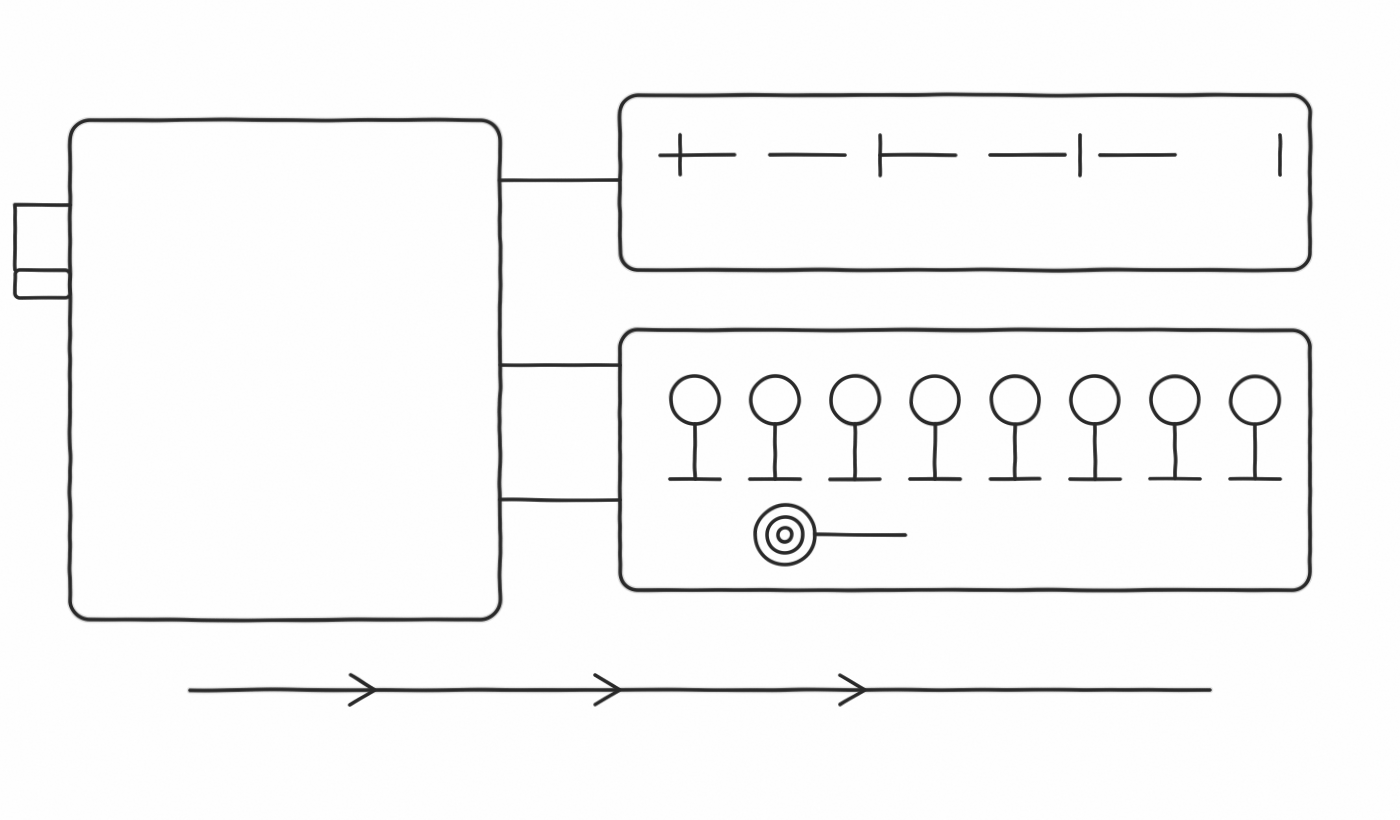
\includegraphics[width=140mm,height=82mm]{029-inert-cue-pencil-base.png}};
  \node[font=\bfseries\large] at (28.5,66) {MEGA 2560};
  \node[font=\small] at (28.5,61) {USB 5 V only};
  \node[font=\small] at (28.5,46) {D22--D29 cue outputs};
  \node[font=\small] at (28.5,41.5) {D30--D34 buttons};
  \node[font=\small] at (28.5,37) {D5--D7 RGB state};
  \node[font=\bfseries\small] at (96.5,68) {FIVE PULL-UP BUTTONS TO GND};
  \foreach \x/\t in {68/REVIEW,79.5/RUN,90/CONFIRM,102/SKIP,114/CANCEL}
    \node[font=\tiny] at (\x,61.5) {\t};
  \node[font=\bfseries\small] at (96.5,50)
    {EIGHT CUE LEDs; ONE 1 kOhm RESISTOR EACH};
  \foreach \x/\n in {69.5/0,77.5/1,85.5/2,93.5/3,101.5/4,109.5/5,117.5/6,125.5/7}
    \node[font=\tiny] at (\x,29.7) {\n};
  \node[font=\scriptsize] at (103,27) {TP29: selected output to Mega GND};
  \foreach \x/\t in {23/review,47.5/confirm,72/visible,96.5/audit}
    \node[font=\scriptsize] at (\x,8.5) {\t};
  \node[font=\scriptsize] at (70,2.2)
    {Orientation only -- inert LED simulator -- no external-load connection};
\end{tikzpicture}
\end{document}
